%
%
%
%
%
%
% Er igang med skrive i denne i forbindelse med feedback fra Anders
%
%
%
%
%
%
%
%
%
%
%
%
%
%
%
%
%
%
%
%
%
\section{Visioner om den samlede forandring}
I dette afsnit beskrives projektgruppens forslag til forbedringer af MinSP. Beskrivelsen er med udgangspunkt i MUST-metodens princip om en samlet vision.
Udover en beskrivelse af den tekniske løsning af forbedringsforslagene, har vi derfor også indraget en vurdering og beskrivelse af behovet for omlægning i arbejdsorganisering, og hvilke konsekvenser, det vil få for sundhedspersonalet. \\
Endelig indgår også en vurdering af hvilke kvalifikationsbehov ændringerne evt. vil medføre.%I dette afsnit ser vi på hvordan visionerne om den samlede forandring, forankres i Regions Sjællands eksisterende version af it-systemet MinSP, dvs. hvordan visionerne skal integreres og anvendes af patienter og sundhedspersonale. \footnote{Professionel it-forundersøgelse, Bødker, Kensing, Simonsen, s. 211} 
\subsection{Teknologi}
I dette afsnit har vi i underpunkterne 'Funktion' og 'Brugergrænseflader' benyttet og anvendt diagnostiske kort \footnote{Bilag 3} til at forstå problemerne vi ønsker løst og ideer til deres løsninger.
%
% ! ER Diagram over de nye funktionalitere / visioner
%
\subsubsection{It-systemer og it-platform}
It-platformen for den samlede vision for MinSP er Sundhedsplatformen.
\\\\
\textbf{Receptfornyelse} \\
It-systemerne er udover MinSP også Sundhedsplatformen og muligvis apotekernes systemer og FMK (det fælles medicin kort), da der skal være integration i mellem disse systemer.\\
Vi har udviklet en prototype for receptfornyelse, der visiualiserer, hvordan en receptfornyelse kan gennemføres.
\\\\
\textbf{Samling af al information} \\
%
% ? - Anders Lassen: "Læring og videnscenter. Der er allerede patienthåndbogen Jeg tror det er out-of-scope":
%
Funktionaliteten vil kunne løses med en 'standardløsning', da der allerede eksisterer flere troværdige informationssider, hvor det er læger, der vedligeholder siderne. \\
Viden og information om diabetes kan slås op i 'Patienthåndbogen'. Der findes allerede et link til 'Patienthåndbogen' i MinSP, men dette link ligger 'gemt' i undermenuen 'Historik' under hovedmenuen 'Sundhedsdata' og ønskes i stedet at være mere fremtrædende. 
\\ 
Under en menu 'Information om dine Diagnoser', kunne et link til 'Patienthåndbogen' placeres. \\
I samme menu kan der lægges et link til 'Diabetesforeningen', der tilbyder fællesskab mellem diabetikere i form af f.eks. motivationsgrupper og diabetescaféer samt rådgivning til diabetikere.
Endvidere kan et link til 'Steno Diabetes Center' give video-information omkring f.eks. 'Hvordan man måler blodglukose', en diætist der fortæller om 'Kulhydrattælling' og informerer om kost og motion, en overlæge, som fortæller om 'Graviditetsdiabetes' m.fl. 
På siden er der også information om blandt andet det at være ny med diabetes, til gravide med diabetes, hjælp til at forstå tal, madopskrifter og meget meget mere. \\
Disse 'standardløsninger' kan være en måde til at løse funktionaliteten 'Samling af al information', og dermed undgås en dyr løsning, hvor hospitalernes sundhedspersonale skal vedligeholde egen udviklede informationssider på MinSP.
\\\\
\textbf{Uniforme Prøvesvar} \\
It-systemerne er udover MinSP også Sundhedsplatformen og FMK, da der skal være integration imellem disse systemer.
\subsubsection{Funktion}
% ? - Indenholde: 'Liste over de enkle it-systemers funktioner'
\textbf{Receptfornyelse}\\
Receptfornyelse skal være integreret i MinSP og Sundhedsplatformen. 
Kravet til funktionaliteten skal være, at patienter i MinSP selv kan aktivere fornyelse af en eller flere recepter for deres ordinerede medicin. 
\\
Receptfornyelsen skal være synlig, som beskrevet i vores diagnostiske kort, og skal derfor placeres som en hovedmenu øverst på MinSP. Undermenuen til hovedmenuen 'Receptfornyelse' skal indeholde: 'Forny recept', 'Medicin kort' og 'Historik'.
\\
Man skal kunne følge gangen i receptfornyelsen fra status 'Medicin bestilt' til 'Medicin kan hentes på apoteket'. Man skal også kunne vælge modtager-apotek med to valgmuligheder, samt om man ønsker en påmindelse om receptfornyelse og i hvilken form (sms, besked i app'en, privat mail eller eboks). 
\\ 
Recepten skal kun kunne fornys, når sidst udleverede dosis er ved slippe op.  
\\
'Medicinkortet' skal indeholde en liste over ordineret medicin.
'Historik' skal indeholde en liste over alle udleveringer af medicin til dato.
\\\\
'Receptfornyelse' er en funktionalitet, der skal ny-udvikles, da der ikke er noget eksisterende funktionalitet, der kan genbruges. Sikkerheden skal være høj i forhold til, at der ikke må udleveres for meget medicin, og det kun er den ordinerede medicin, der må fornys. \\
I statuslinje for gangen i receptfornyelsen, skal registreringen overføres af sundhedspersonalet fra Sundhedsplatformen til MinSP.\\
Modtagerapotek skal kunne vælges i forhold til bopæl. Det vil kræve en tabel med data over hvor alle apoteker i Region Sjælland ligger.\\
Påmindelse vil kræve, at der beregnes en dato for fornyelse af recept i forhold til sidste fornyelse. Hertil skal bruges databaser med oplysninger om ordineret medicin, historikken for udleveret medicin og receptfornyelser. Vi forudsætter, at databaser med disse oplysninger allerede findes i FMK, men at der skal laves integration med disse databaser. \\
\\
Jf. mail-interview med Mette Christensen, MinSP projektkonsulent, Region Sjælland,\footnote{Bilag 7} er der ikke etableret integration mellem MinSP og FMK. Mette Christensen oplyser, at Region Sjælland selv har arbejdet med at finde en alternativ løsning, men at dette har været en kompliceret opgave og er ikke løst endnu. \\
Ligeledes kan recepter, uden integration med FMK, ikke gøres tilgængelig alle steder, som det ellers ville kunne i receptdatabasen i FMK.\footnote{Anders Lassen, ekstern lektor, DIKU: "Det er praksis, at recepter lægges ud på receptdatabase, så den er tilgængelig alle steder. FMK kan det."} Derfor skal Patienttabellen i databasen for MinSP  udvides til at kunne gemme oplysninger om 'Primær apotek' og 'Sekundær apotek', som det gøres i sundhed.dk, jf. oplysning fra praktiserende læge Christian von der Osten i Greve, som vi har lavet en markedsundersøgelse med.\\ 
På baggrund af ovennævnte beskrivelse vurderer vi, at 'Receptfornyelse' er en kompliceret funktionalitet at udvikle.
\\\\
\textbf{Samling af al information} \\
Et forslag til at imødekomme forbedringsforslaget om en 'Samling af al information' kunne være, at tilføje en undermenu 'Information om dine diagnoser' under hovedmenuen Profil. Under denne undermenu kan der placeres link til relevante og ankerkendte lægefaglige udviklede sider som f.eks. Patienthåndbogen, Diabetesforeningen og Steno Diabetes Center. Siderne kan, som vist i mock-up's for dette forbedringsforslag, være opdelt efter patientens diagnoser. Løsningen er fleksible, da det vil være nemt at tilføje flere links. Beslutningen om hvilke links patienterne skal tilbydes, skal ske på baggrund af konsensus mellem alle hospitaler i Region Sjælland. 
\\\\ 
\textbf{Uniforme Prøvesvar} \\
Denne funktionalitet vil kunne løses ved, at man til hvert enkelt prøvesvar knytter en forklaring af prøve-typen på dansk. Der skal her udover angives, hvor prøven er taget (navn på hospital, læge eller laboratorie).\\
Prøvesvarene skal holdes adskilt pr. diagnoses, hvis patienten har flere diagnoser.\\
I databasen for MinSP skal tabel med prøvesvar udvides til at kunne gemme forklarende tekst på dansk, om hvad prøven viser, navn på hospital / læge / laboratori, samt hvor prøven er taget. Derfor skal der også oprettes en tabel med hospitals- / læge- / laboratorie navne, som de pågældende navne kan hentes fra.\\ 
Tekstbeskrivelsen kan være en standardtekst pr. prøvetype, mens navet på stedet og hvor prøven er taget, kan variere. Dette skal derfor indrapporteres af personalet, når prøvesvar indrapporteres. \\
For at kunne holde prøvesvar adskilt pr. diagnose, skal tabellen med prøvesvar, i databasen for MinSP, udvides til at kunne gemme oplysninger om diagnose. Sundhedspersonalet skal for hvert prøvesvar indrapportere relevant diagnose for prøvesvaret. 
\subsubsection{Brugergrænseflader} % Krav til Brugergrænseflader
Brugergrænsefladerne skal designes så de overholder GUI-guidelines for god interaktionsdesign. %  Benyon s. 88 
\\\\
\textbf{Receptfornyelse} \\
Implementering af receptfornyelses funktionaliteten vil kræve integration med Sundhedsplatformens medicinmodul og apotekerenes systemer. 
Der skal være en ny grænseflade mellem MinSP og SP. \\\\
Forslag til brugergrænseflade for patienten fremgår af nedenstående Mock-up's. \\
\\
Designet er udarbejdet på baggrund af inspiration af designet i sundhed.dk, som vi har fået fremvist af praktiserende læge Christian von der Osten i Greve, som vi har lavet en markedsundersøgelse med.\\
\begin{figure}[H]
	\centering
	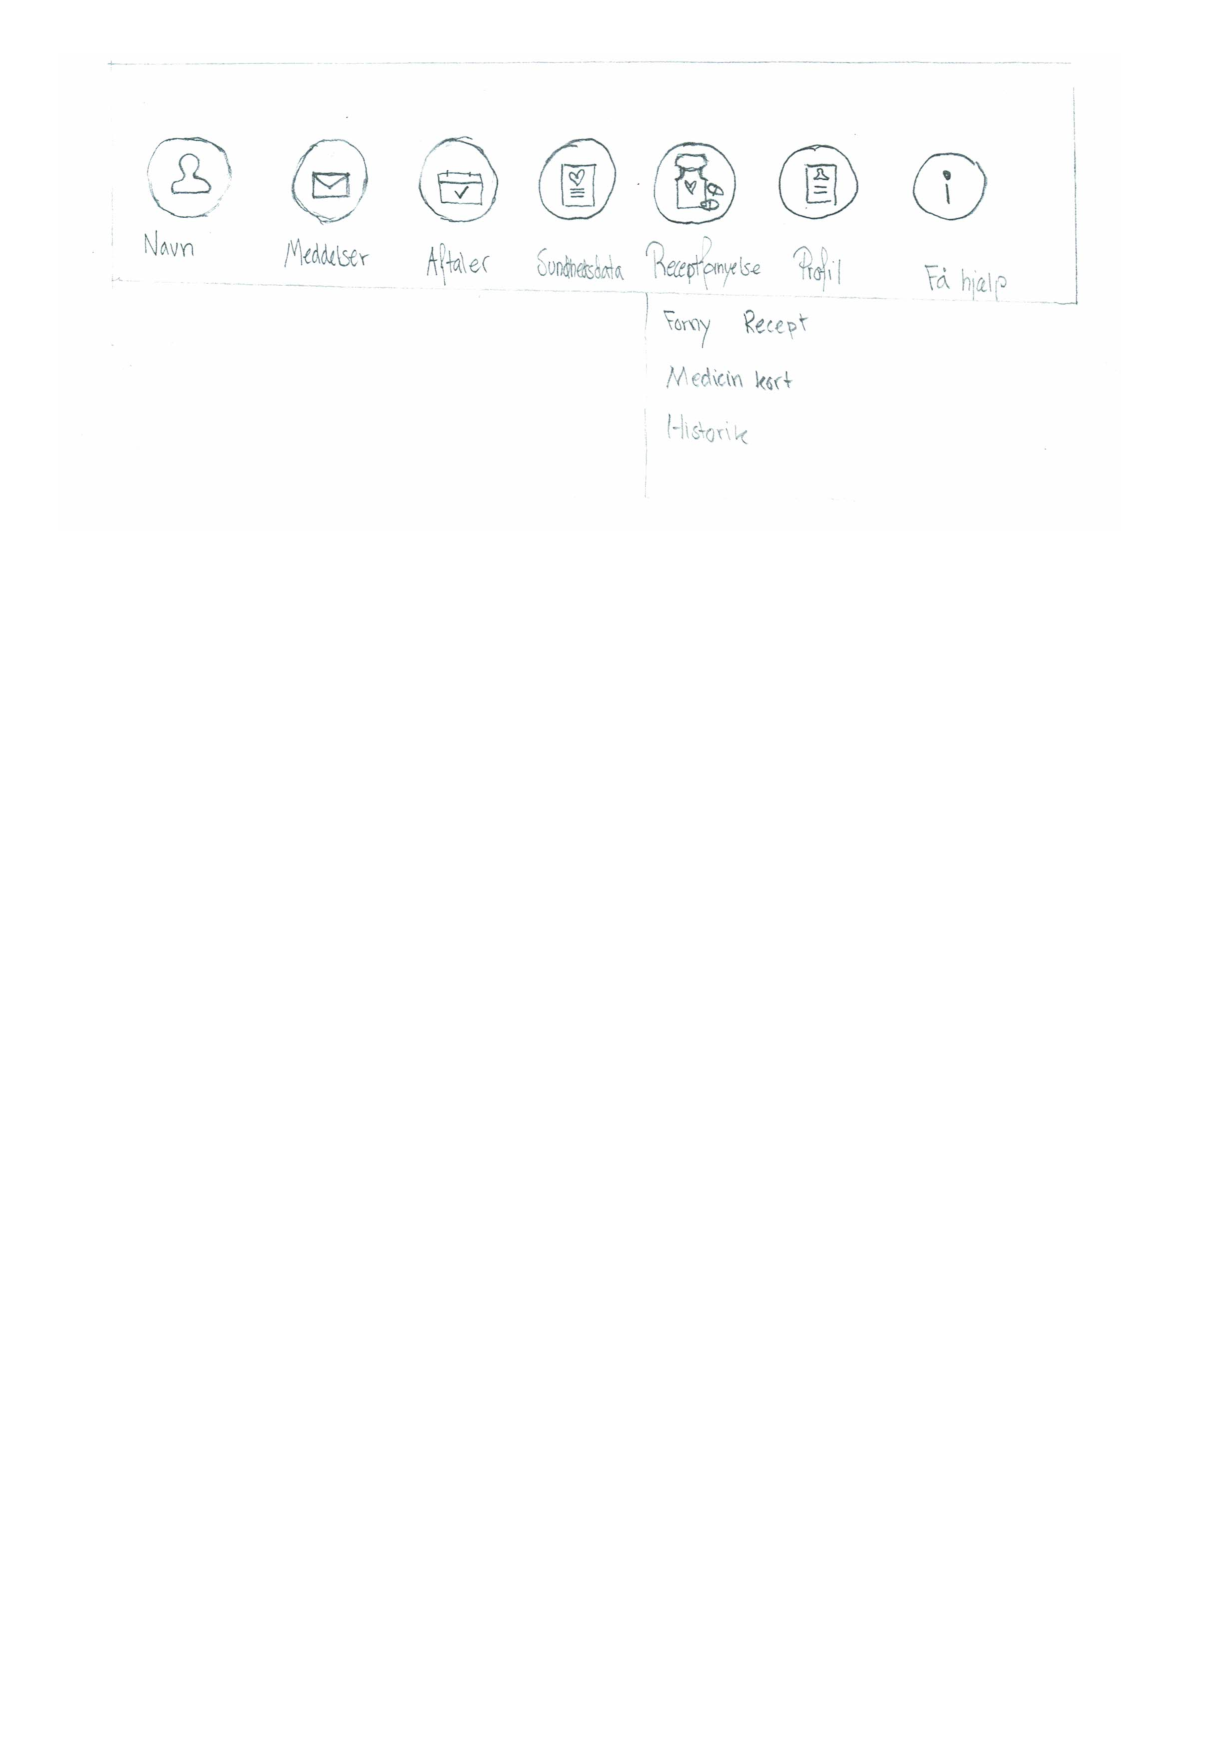
\includegraphics[angle=0, width=\linewidth]{Materials/FornyRecept_Hovedmenu.pdf}
	\caption{Mock-up for modulet 'Receptfornyelse': Hovedmenuen}
	\label{fig:Mock-Up1}
\end{figure}
Mock-up'en til Hovedmenuen med et 'Receptfornyelses-menu' er lavet med inspiration fra vores scenarier.\footnote{Bilag 5}
\begin{figure}[H]
	\centering
	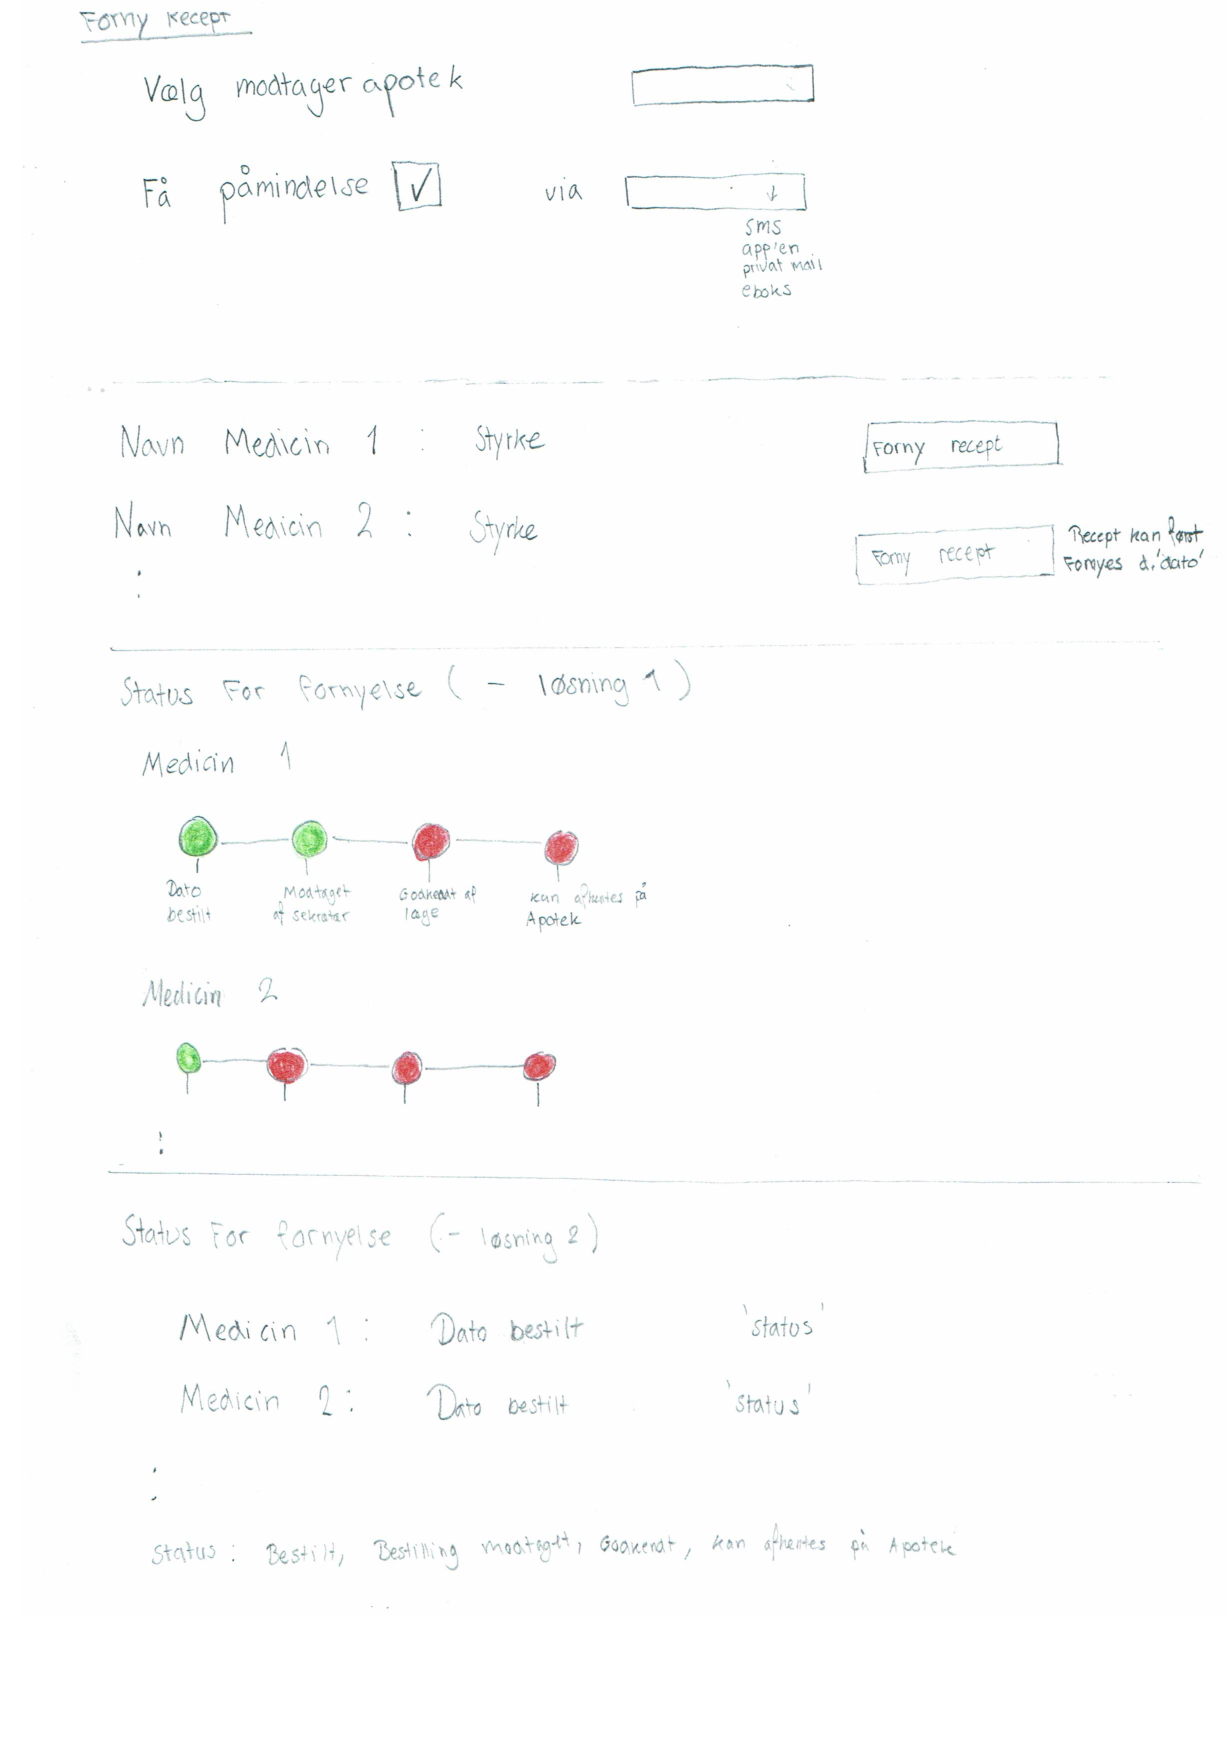
\includegraphics[angle=0, width=\linewidth]{Materials/FornyRecept.pdf}
	\caption{Mock-up for modulet 'Receptfornyelse': Undermenu, 'Forny recept'}
	\label{fig:Mock-Up2}
\end{figure}
I 'Vælg modtagerapotek' skal man i en drop-down menu kunne vælge mellem de to apoteker, som er tættest på en.\\
Hvis patienten ønsker påmindelse om receptfornyelse, skal patienten sætte hak ved 'Få påmindelse'.\\
Bemærk at knappen 'Forny recept' skal være blokeret i perioden, hvor recepten ikke må fornys. Der skal udover indformeres om, hvornår patienten igen kan forny sin recept, med tekst ved siden af 'Forny recept'-knappen som vist i mock-up'en. Denne funktionalitet findes ikke i sundhed.dk.\\
Når patienten fornyer sin recept, kan der være en fortrydelsesbesked, som siger: 'Er du sikker på du vil forny din recept?' hvor man skal kunne vælge 'Ja' eller 'Nej.\\
Der er to forslag til måden, hvorpå status for fornyelse kan vises.  Statusmulighederne i løsning to er: Bestilt, bestilling modtaget, godkendt og kan afhentes på Apotek. Denne løsning er inspireret af designet på sundhed.dk.\\
\begin{figure}[H]
	\centering
	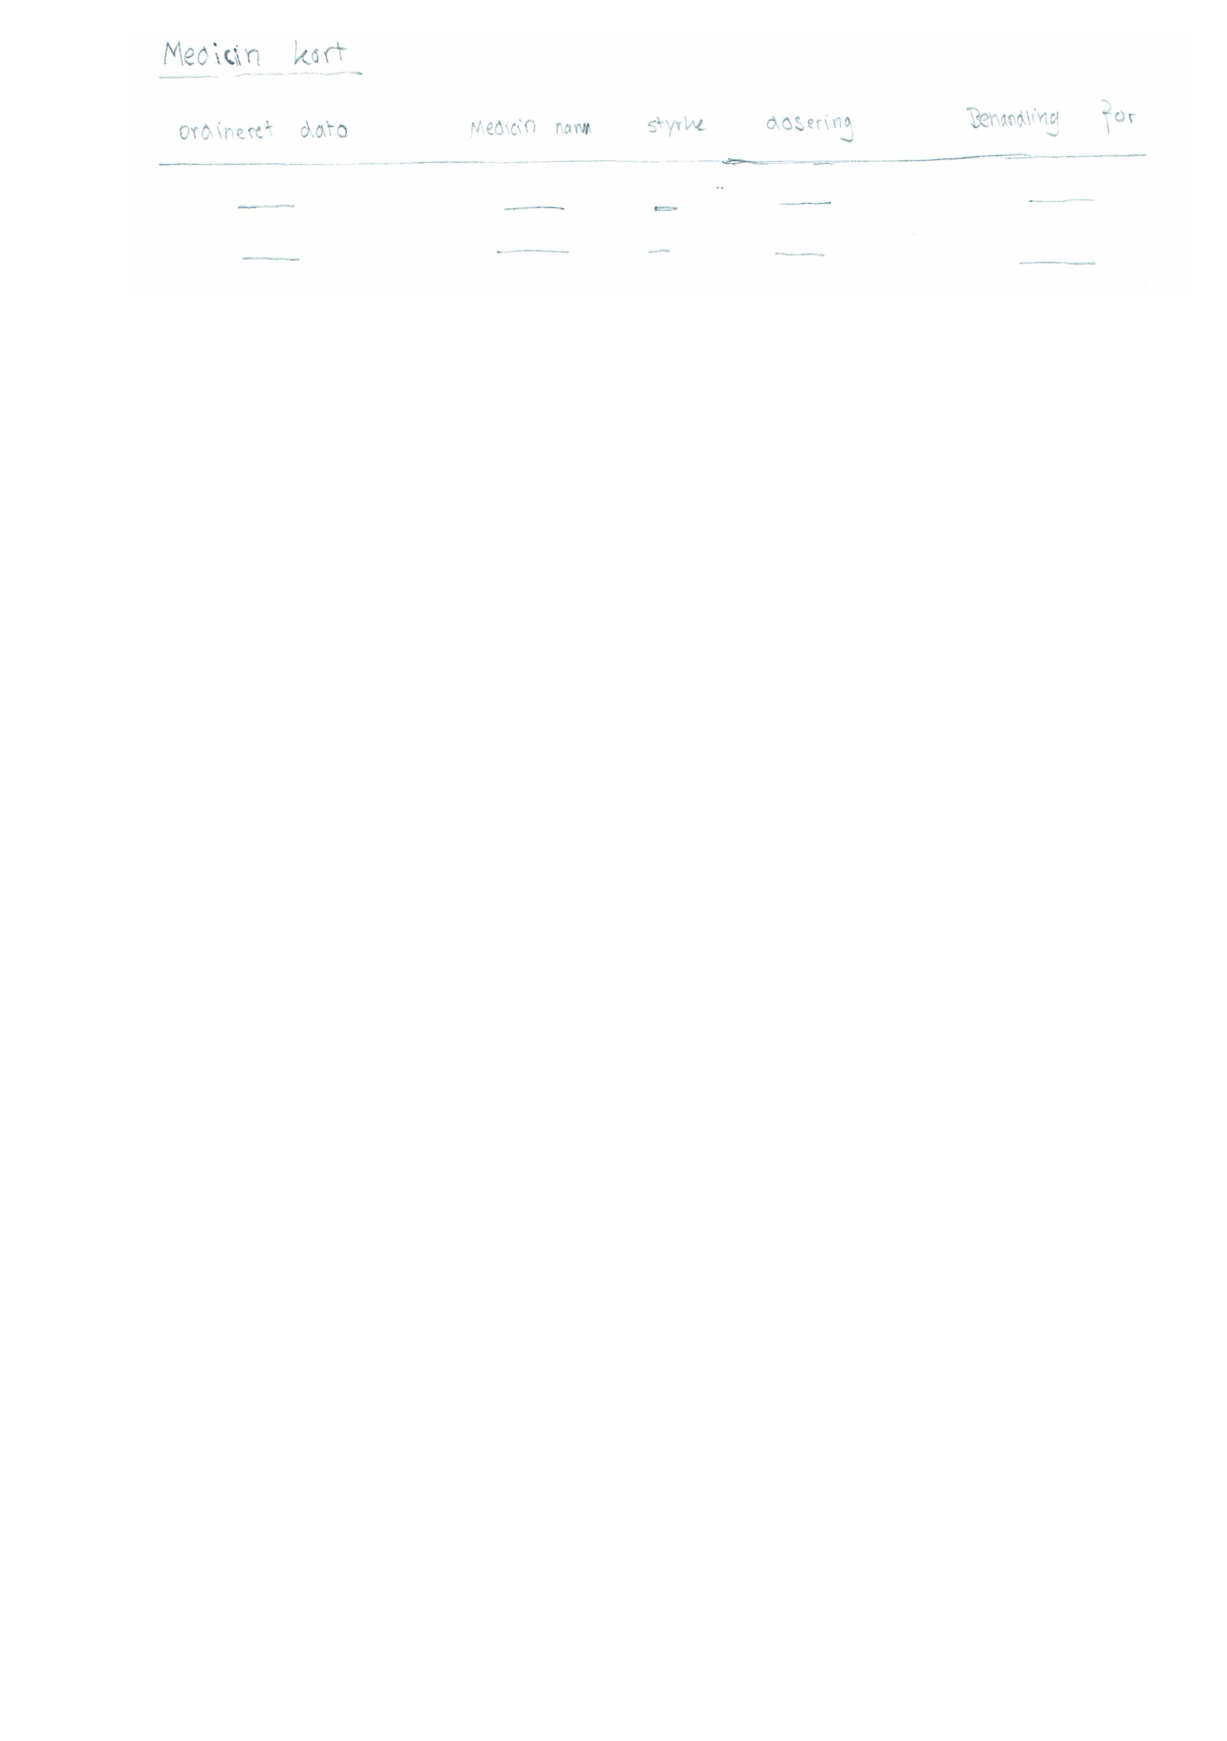
\includegraphics[angle=0, width=\linewidth]{Materials/FornyRecept_Medicinkort.pdf}
	\caption{Mock-up for modulet 'Receptfornyelse': Undermenu, 'Medicin kort'}
	\label{fig:Mock-Up3}
\end{figure}
\begin{figure}[H]
	\centering
	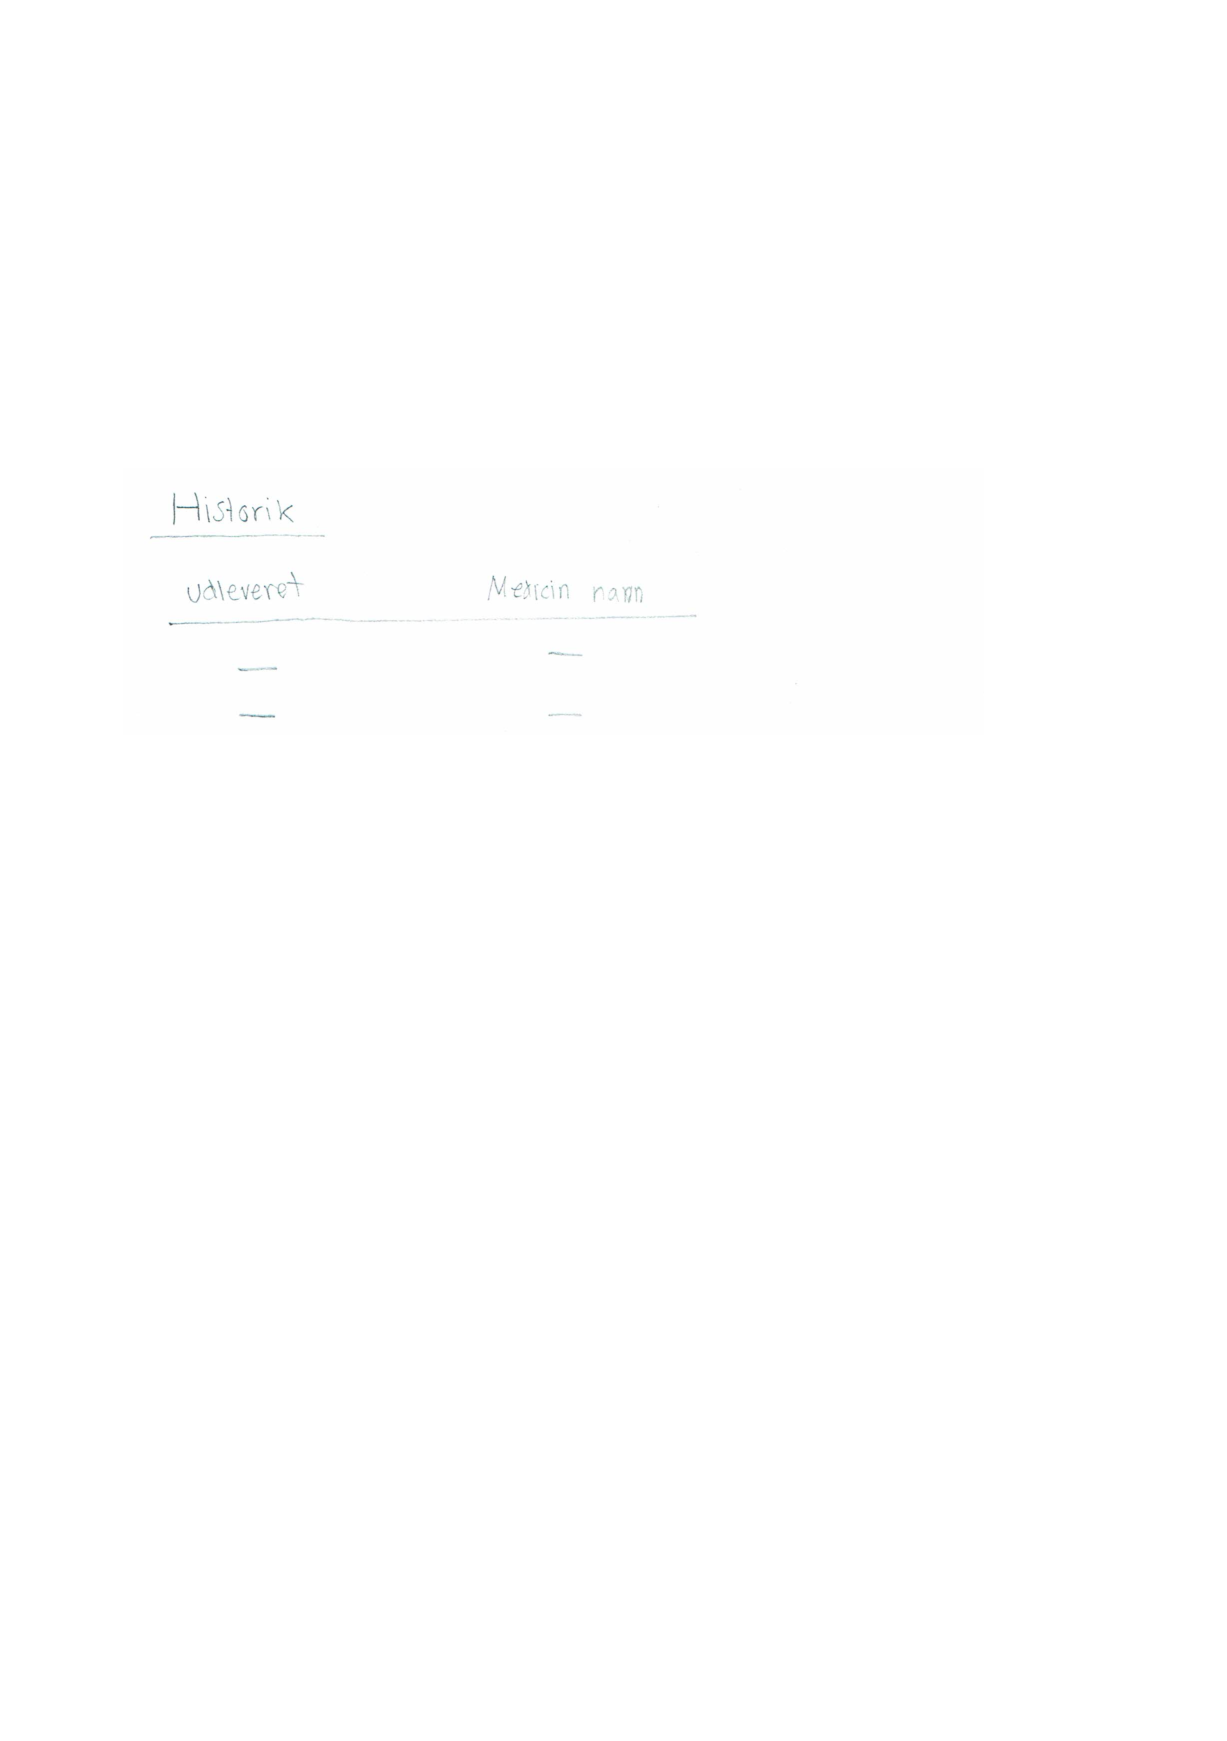
\includegraphics[angle=0, width=\linewidth]{Materials/FornyRecept_Historik.pdf}
	\caption{Mock-up for modulet 'Receptfornyelse': Undermenu, 'Historik'}
	\label{fig:Mock-Up4}
\end{figure}
% ? - Scenarios
\textbf{Samling af al information} \\
Forslag til brugergrænseflade for patienten fremgår af nedenstående Mock-up's:\\
\begin{figure}[H]
	\centering
	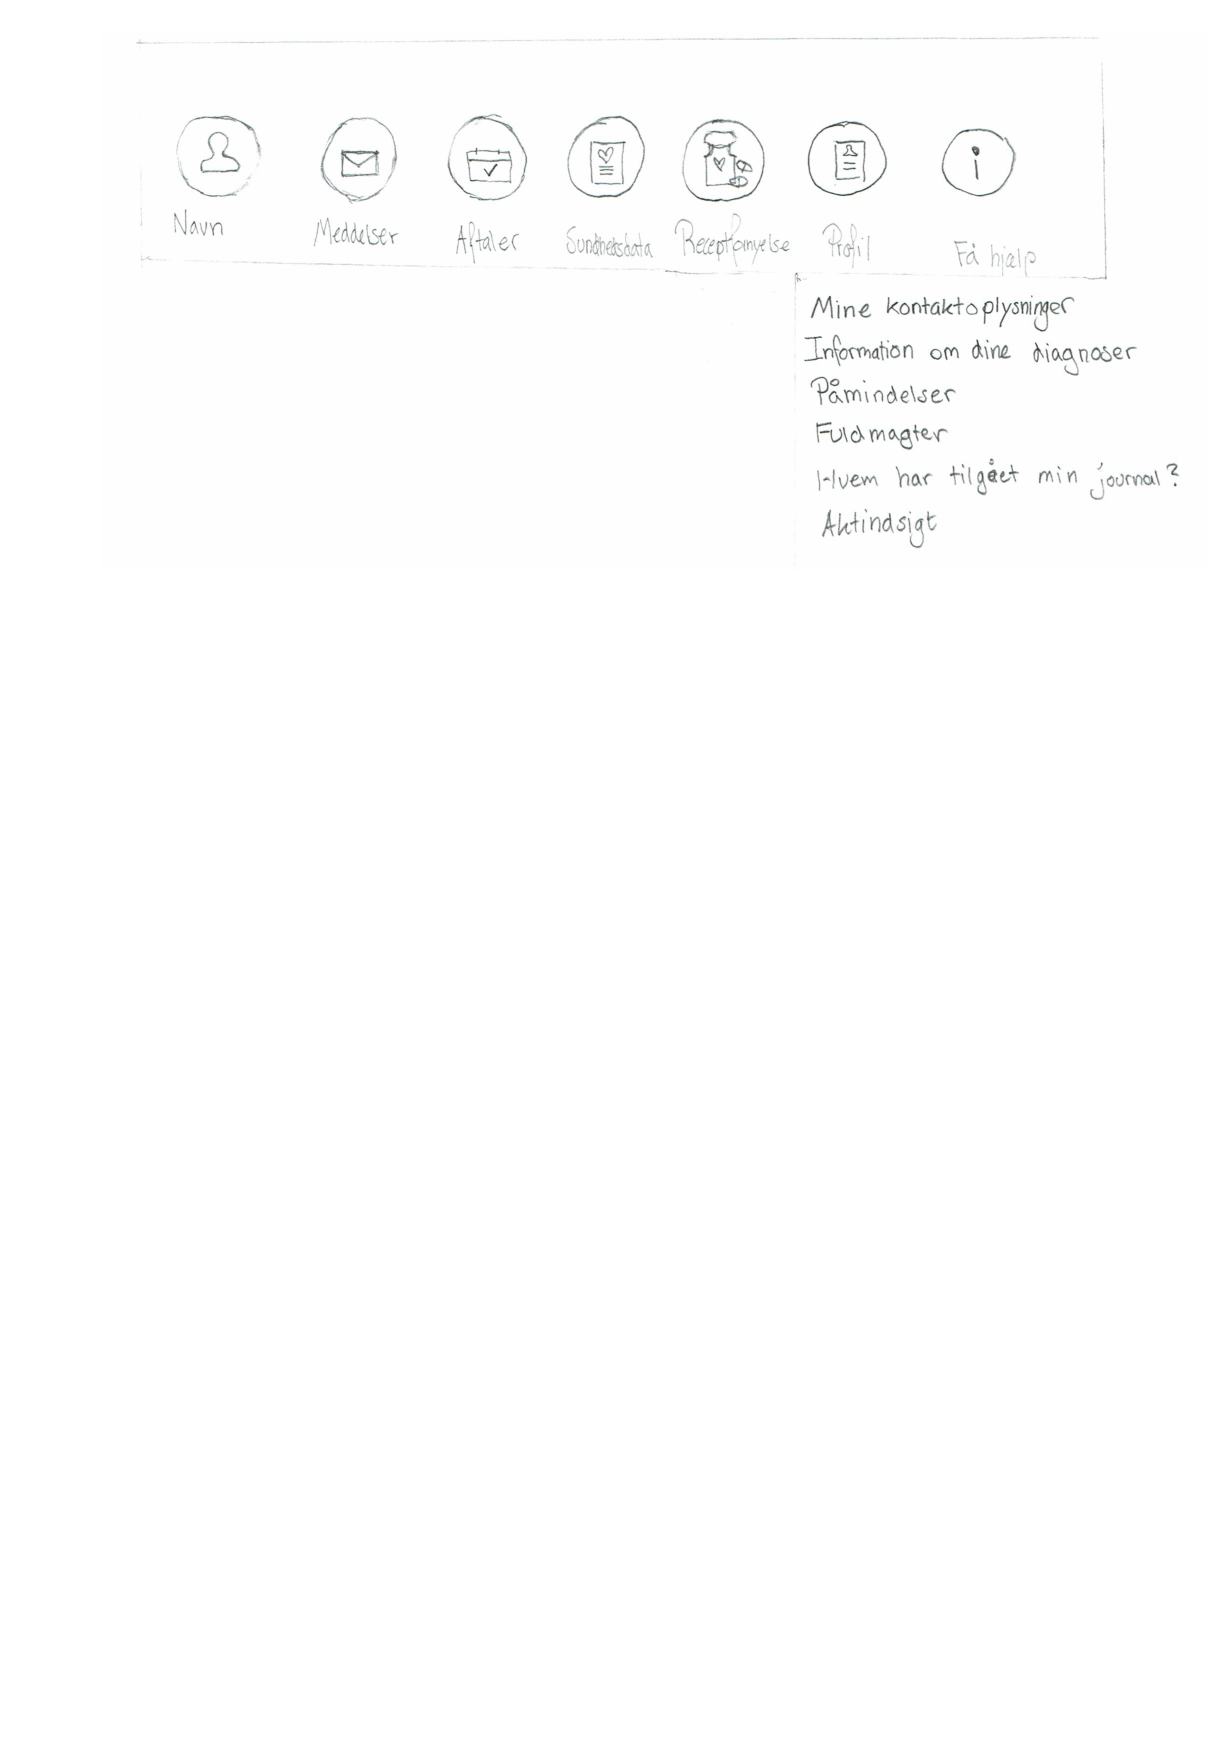
\includegraphics[angle=0, width=\linewidth]{Materials/Information_Hovedmenu.pdf}
	\caption{Mock-up for modulet 'Information om dine diagnoser': Hovedmenu, 'Profil'}
	\label{fig:Mock-Up5}
\end{figure}
Der er i hovedmenuen Profil tilføjet undermenuen 'Information om dine diagnoser'.
\begin{figure}[H]
	\centering
	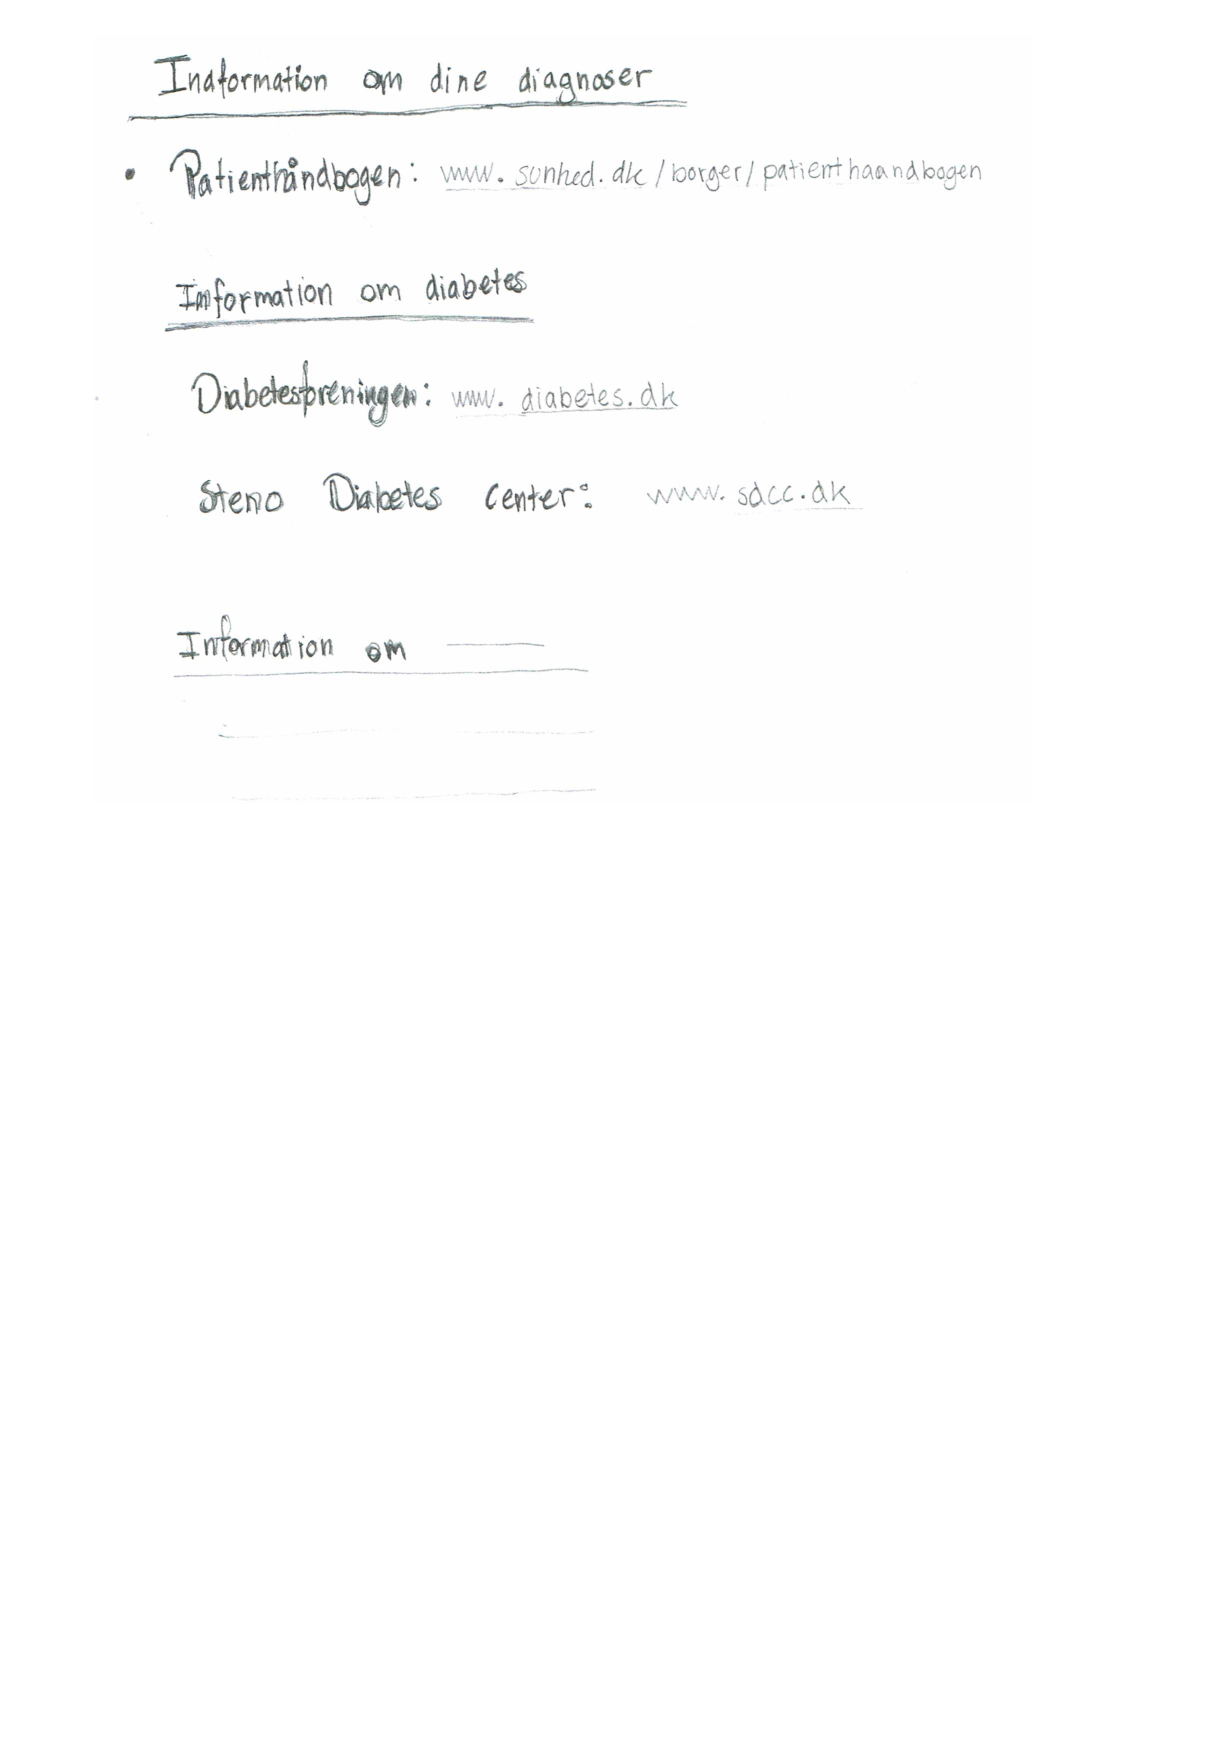
\includegraphics[angle=0, width=140mm]{Materials/Info2.pdf}
	\caption{Mock-up for modulet 'Information om dine diagnoser': Undermenu}
	\label{fig:Mock-Up6}
\end{figure}
Her kan patienten søge generel infomation om sin/sine diagnoser via links til relevante og anerkendte hjemmesider, der er udarbejdet af sundhedsfagligt personale.\\\\
\textbf{Uniforme Prøvesvar} \\
Forslag til brugergrænseflade for patienten fremgår af nedenstående Mock-up's:\\
\begin{figure}[H]
	\centering
	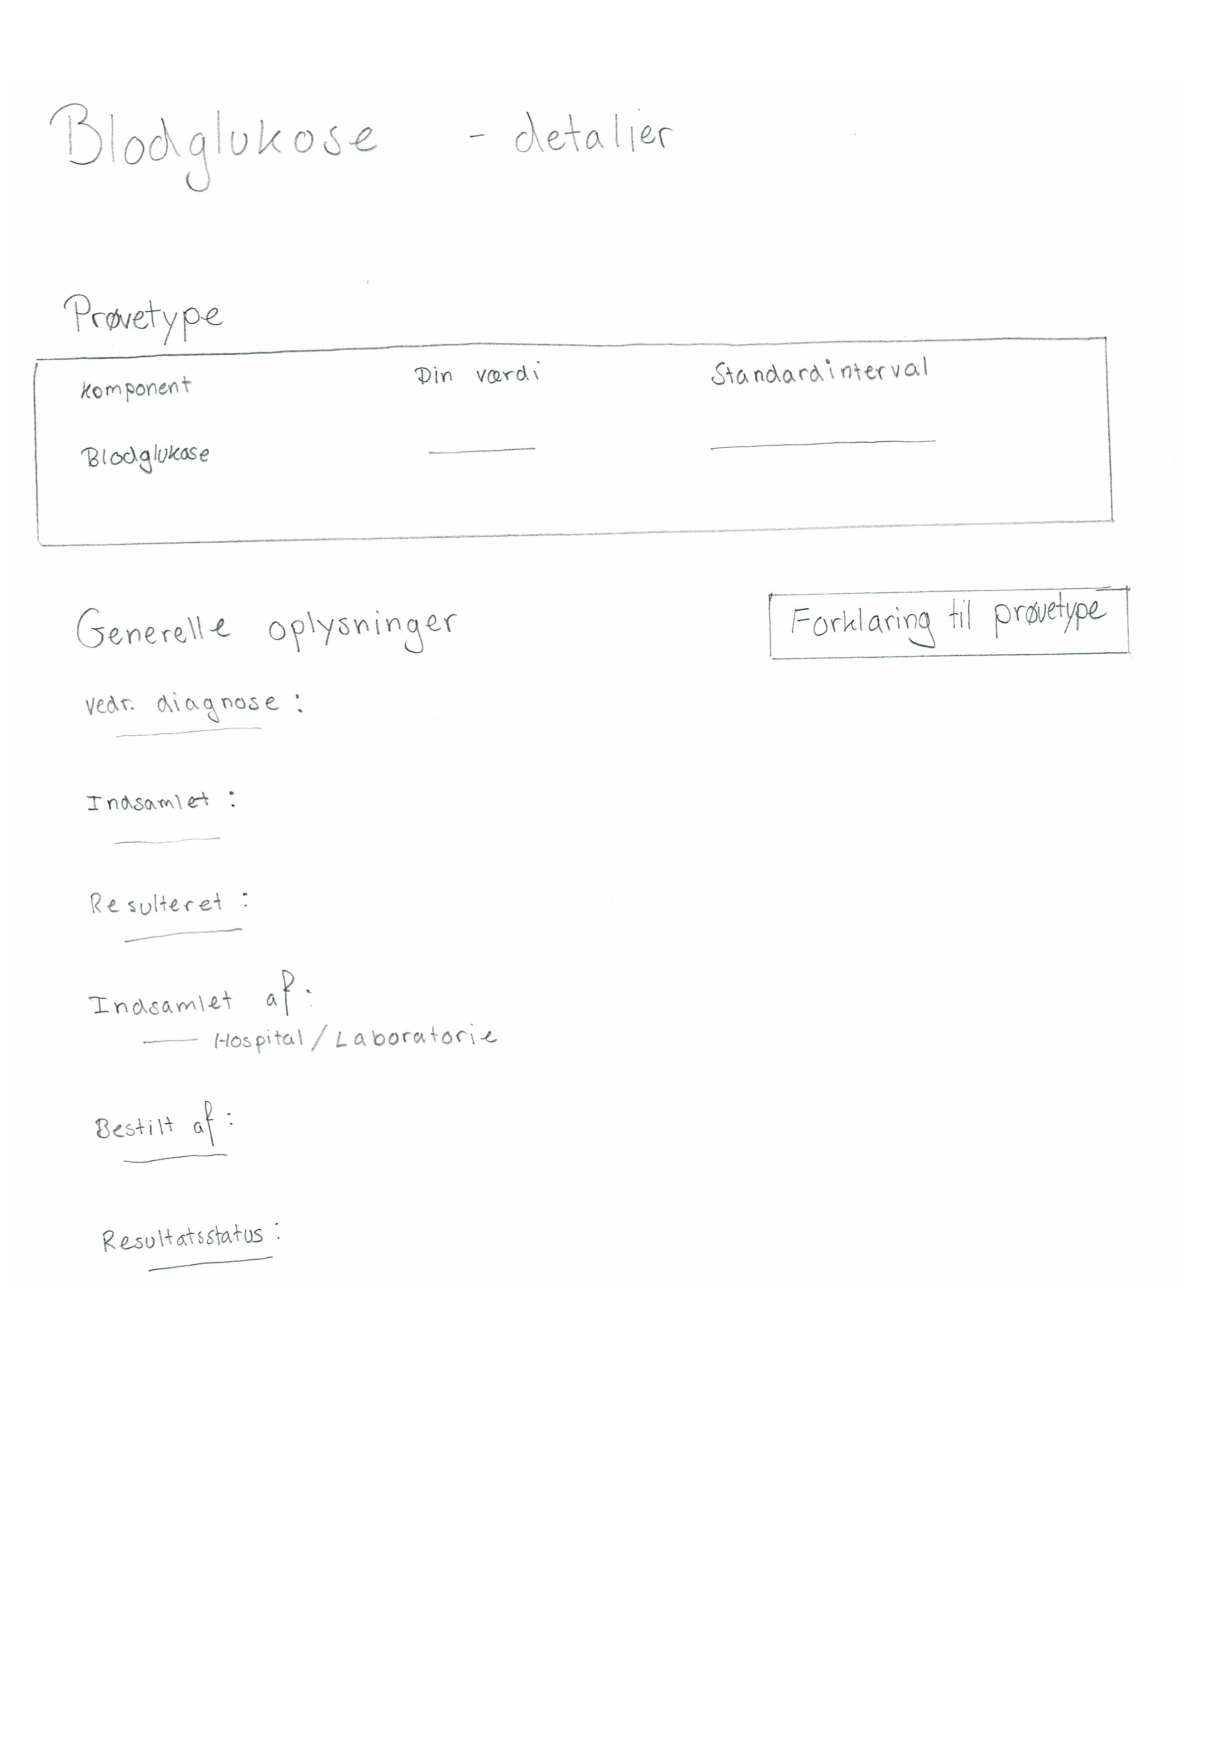
\includegraphics[angle=0, width=140mm]{Materials/provesvar.pdf}
	\caption{Mock-up for modulet 'Prøvesvar'}
	\label{fig:Mock-Up7}
\end{figure}
Når patienten klikker på knappen 'Forklaring til prøvetype' skal der vises en tekst på dansk med forklaringen til prøvetypen. Det kan laves som en pop-up eller ny side.
\subsection{Arbejdets organisering} 
Det lykkedes os desværre ikke at få mulighed for at foretage virksomhedsbesøg. \footnote{Dybdeanalyse, afsnit 5 Konsekvensanalyse s. 18} Virksomhedsbesøg ville have givet os mulighed for at observere sundhedspersonalets nuværende arbejdspraksis, når patienterne fornyer deres recept via besked funktionen i MinSP og får taget prøver og givet prøvesvar.\\ 
Vi ville derfor bedre have kunnet vurdere hvilke ændringer der var behov for, i forhold til arbejdsorganiseringen for sundhedspersonalet og arbejdsfordelingen imellem læge, lægesekretærer, laboranter m.fl, og vi ville dermed have haft et bedre grundlag for at vurdere fordele og ulemper for sundhedspersonalet og relationerne imellem dem, deres arbejdsgange og evt. kvalifikationsbehov ved implementering af vores forbedringsforslag.\\
Vi har derfor ikke haft den viden, som MUST-metodens princip om, at arbejdspraksis, skal opleves ellers kunne have givet os. Dog har vi via mail-interviews med Katrine Bundgaard Kaalund, Sundhedsplatform teamet på NOH \footnote{Bilag 6} og  Mette Christensen, MinSP projektkonsulent, Region Sjælland \footnote{Bilag 7} fået lidt viden herom. \\
Vi har også, her i fornyelsesfasen, haft mulighed for at lave en markedsundersøgelse om sundhed.dk ved besøg hos praktiserende læge Christian von der Osten i Greve. Her har vi fået gennemgået og forklaret receptfornyelses funktionen i sundhed.dk, som er det system lægen bruger til receptfornyelse. Vi har derfor haft mulighed for at observere forretningsgangen i receptfornyelse i sundhed.dk og fået inspiration til vores udvikling af receptfornyelse i MinSP.\\\\
\textbf{Receptfornyelse} \\
En automatisk receptfornyelse, som i sundhed.dk, som vist hos læge Christian von der Osten, vil ændre arbejdsgangen for sundhedspersonalet. \\ 
Jf. Katrine Bundgaard Kaalund, Sundhedsplatform teamet på NOH \footnote{Bilag 6}, skal lægen fortsat stadigvæk tjekke, at ordineringen er korrekt i forhold til journalen, men læge-sekretæren vil muligvis slippe for involvering i arbejdsgangen af receptfornyelse i forhold til at skulle forberede recepten til lægen, forudsat at det nye receptfornyelses modul vil kunne klare det.\\
Jf. Mette Christensen, MinSP projektkonsulent, Region Sjælland, \footnote{Bilag 7} vil læge-sekretæren ikke skulle bruge tid på at undersøge hvilken afdelingen recepten hører til, og hvilken læge der så skal godkende, forudsat at systemet kan spore hvilken læge, der har givet recepten første gang.\\
Læge-sekretæren slipper også for at skrive besked tilbage til patienten, da patienten nu selv kan se forløbet i statuslinjen.
\\\\
\textbf{Samling af al information} \\
Hvis funktionaliteten implementeres via vores løsningsforslag med links, vil der ikke være nogen ændringer til arbejdsgange og arbejdets organisering. \\
Hvis funktionaliteten skulle have været implementeret som en ny-udviklet informationsside, ville det være sundhedspersonalet, der skulle skrive alt informationen/optage videoer mv., og siden ville skulle vedligeholdes af sundhedspersonalet, så det ville være en ekstra opgave, som sundhedspersonalet (læger, diætister og sygeplejeskær m.fl.) herved bliver pålagt. 
\\\\
\textbf{Uniforme Prøvesvar} \\
Implementering af denne funktionalitet vil give ekstra arbejde for lægesekretæren eller laboratorie medarbejdere i forhold til indrapporteringen af prøvesvar, da der vil være flere informationer (navn på sted hvor prøven er taget og navn på diagnose), der skal indtastes, end med nuværende løsning. Der vil forinden være ekstra arbejde for lægen, da det er denne, der skal informere laboratorie-personalet eller lægesekretæren om, hvilken diagnose, de enkle prøvesvar vedrører.\\
Der skal tages stilling til hvor i organisationen indrapporteringen skal foretages. Desuden skal der nedsættes et udvalg enten på regionalt eller på landsplan, som skal udarbejde standardsvarene til de uniforme prøvesvar.
\subsection{Kvalifikationsbehov}
\textbf{Receptfornyelse} \\
Receptfornyelses funktionaliteten vil ikke kræve nogen større oplæring af sundhedspersonalet, hvis de er rutinerede brugere af Sundhedsplatformen, men blot en introduktion til, hvordan den nye funktionalitet fungerer, så de kan vejlede patienterne i brugen.
\\\\
\textbf{Samling af al information} \\
Da funktionaliteten implementeres via links, vil det ikke kræve nogen oplæring af sundhedspersonalet. Sundhedspersonalet skal dog have kendskab til indholdet, af de sider, der linkes til, så de kan informere patienterne om den mulighed, de har for selv at søge information her, og så de også selv kan drage nytte af det i deres vejledning af patienter.
\\\\
\textbf{Uniforme Prøvesvar} \\
Vores vurdering er, at ændringerne ikke kræver ekstra kvalifikationer, da ændringen for sundhedspersonalet består i data-indtastning, som vi forudsætter at de allerede er bekendt med.\\\\
Da vi ikke har haft mulighed for kontakt med sundhedspersonalet i nogen af Region Sjællands hospitaler, har vi ikke haft mulighed for løbende at kunne informere personalet og ledelsen om vores forbedringsforslag af MinSP, som vi har arbejdet med i dette forundersøgelses projekt. Vi har derfor ikke til fulde kunnet opfylde MUST-metodens princip om forankring, hvor man fra forundersøgelsens første fase skal skabe forståelse og opbakning ved løbende at informere alle interessenter, der senere vil blive berørt af forandringerne. Det gælder både ledelse, sundhedspersonale og dem, der skal være ansvarlige for den tekniske og organisatoriske implementering.
